%%%%%%%%%%%%%%%%%%%%%%%%%%%%%%%%%%%%%%%%%%%%%%%%%%%%%%%%%%
% # Reanalysis of the Processing Data with RP Acceptors Removed
%%%%%%%%%%%%%%%%%%%%%%%%%%%%%%%%%%%%%%%%%%%%%%%%%%%%%%%%%%

\chapter{Reanalysis of the Processing Data with RP Acceptors Removed}\label{ch-reanalysis}

This chapter investigates whether it was the consistent acceptors of resumptive RCs who were primarily responsible for the by-group processing effects for resumption observed in the EPT and the SPRT. To do this, I~first removed consistent RP acceptors and then reran three of the main EPT and SPRT analyses. Section \ref{rnl-rq} lists my research questions (RQs) for the chapter. Section \ref{rnl-acceptor} describes how consistent RP acceptors were identified and removed from the ORC and SRC datasets. Sections \ref{rnl-ept-token}--\ref{rnl-spr-accuracy} examine the results, addressing the RQs one at a time. Section \ref{rnl-conclusion} concludes the chapter.

%========================================================%
\section{Research questions}\label{rnl-rq}
%========================================================%

My research questions for the chapter were as follows:

\begin{enumerate}[\bfseries RQ1:,itemsep=5pt]
\item {\bfseries With RP acceptors removed, how does processing strain affect rates of resumptive RCs in the EPT?}\par\nobreak
Prediction: Rates of resumption responses will increase down the SLW hierarchy (from short-distance to long-distance to \textit{wh}-island). This would indicate that resumption eases RC production under processing strain, even for participants who do not generally accept resumptive RCs.
\end{enumerate}\vspace{5pt}

\begin{enumerate}[\bfseries RQ2:,itemsep=5pt]
\item {\bfseries With RP acceptors removed, how does resumption in RCs affect RTs at the regions of interest in the SPRT?}\par\nobreak
Prediction: RTs following RPs will be faster than RTs following gaps at lower levels on the SLW hierarchy. Such a result would suggest that resumption facilitates RC comprehension when there is strain on the processor, even for participants who do not accept RPs.
\end{enumerate}\vspace{5pt}

\begin{enumerate}[\bfseries RQ3:,itemsep=5pt]
\item {\bfseries With RP acceptors removed, how does resumption affect comprehension-question accuracy in the SPRT?\footnotemark{}}\par\nobreak
Prediction: Accuracy will be higher for RP trials than for gap trials, at least at lower levels on the SLW hierarchy. This would show that resumption assists with accurate RC interpretation when processing load is high, even for participants who do not accept RPs.
\end{enumerate}\vspace{5pt}

\footnotetext{It would also have been possible to look at the comprehension-question RTs from the SPRT (see~Section~\ref{spr-qrt}); however, I~decided to limit analyses in this chapter to one type of data from the EPT and two types of data from the SPRT.}

%========================================================%
\section{Identifying RP acceptors}\label{rnl-acceptor}
%========================================================%

Recall from Chapter~\ref{ch-ajt} that participants who gave high acceptability ratings (4, 5, or 6) to ≥~80\% of RP trials in at least one English AJT condition were identified as `RP acceptors' (henceforth, the RP acceptor subgroup). For the present analyses, all other participants were classified as `RP non-acceptors' (henceforth, the RP non-acceptor subgroup). Figure~\ref{fig:ajt-prop-subgroup} shows the relative proportions of RP acceptors and RP non-acceptors in the ORC and SRC datasets.

\begin{figure}
\caption{Proportion of RP acceptors and RP non-acceptors in the ORC and SRC English acceptability judgment tasks} \label{fig:ajt-prop-subgroup}
\raggedright\setstretch{1}
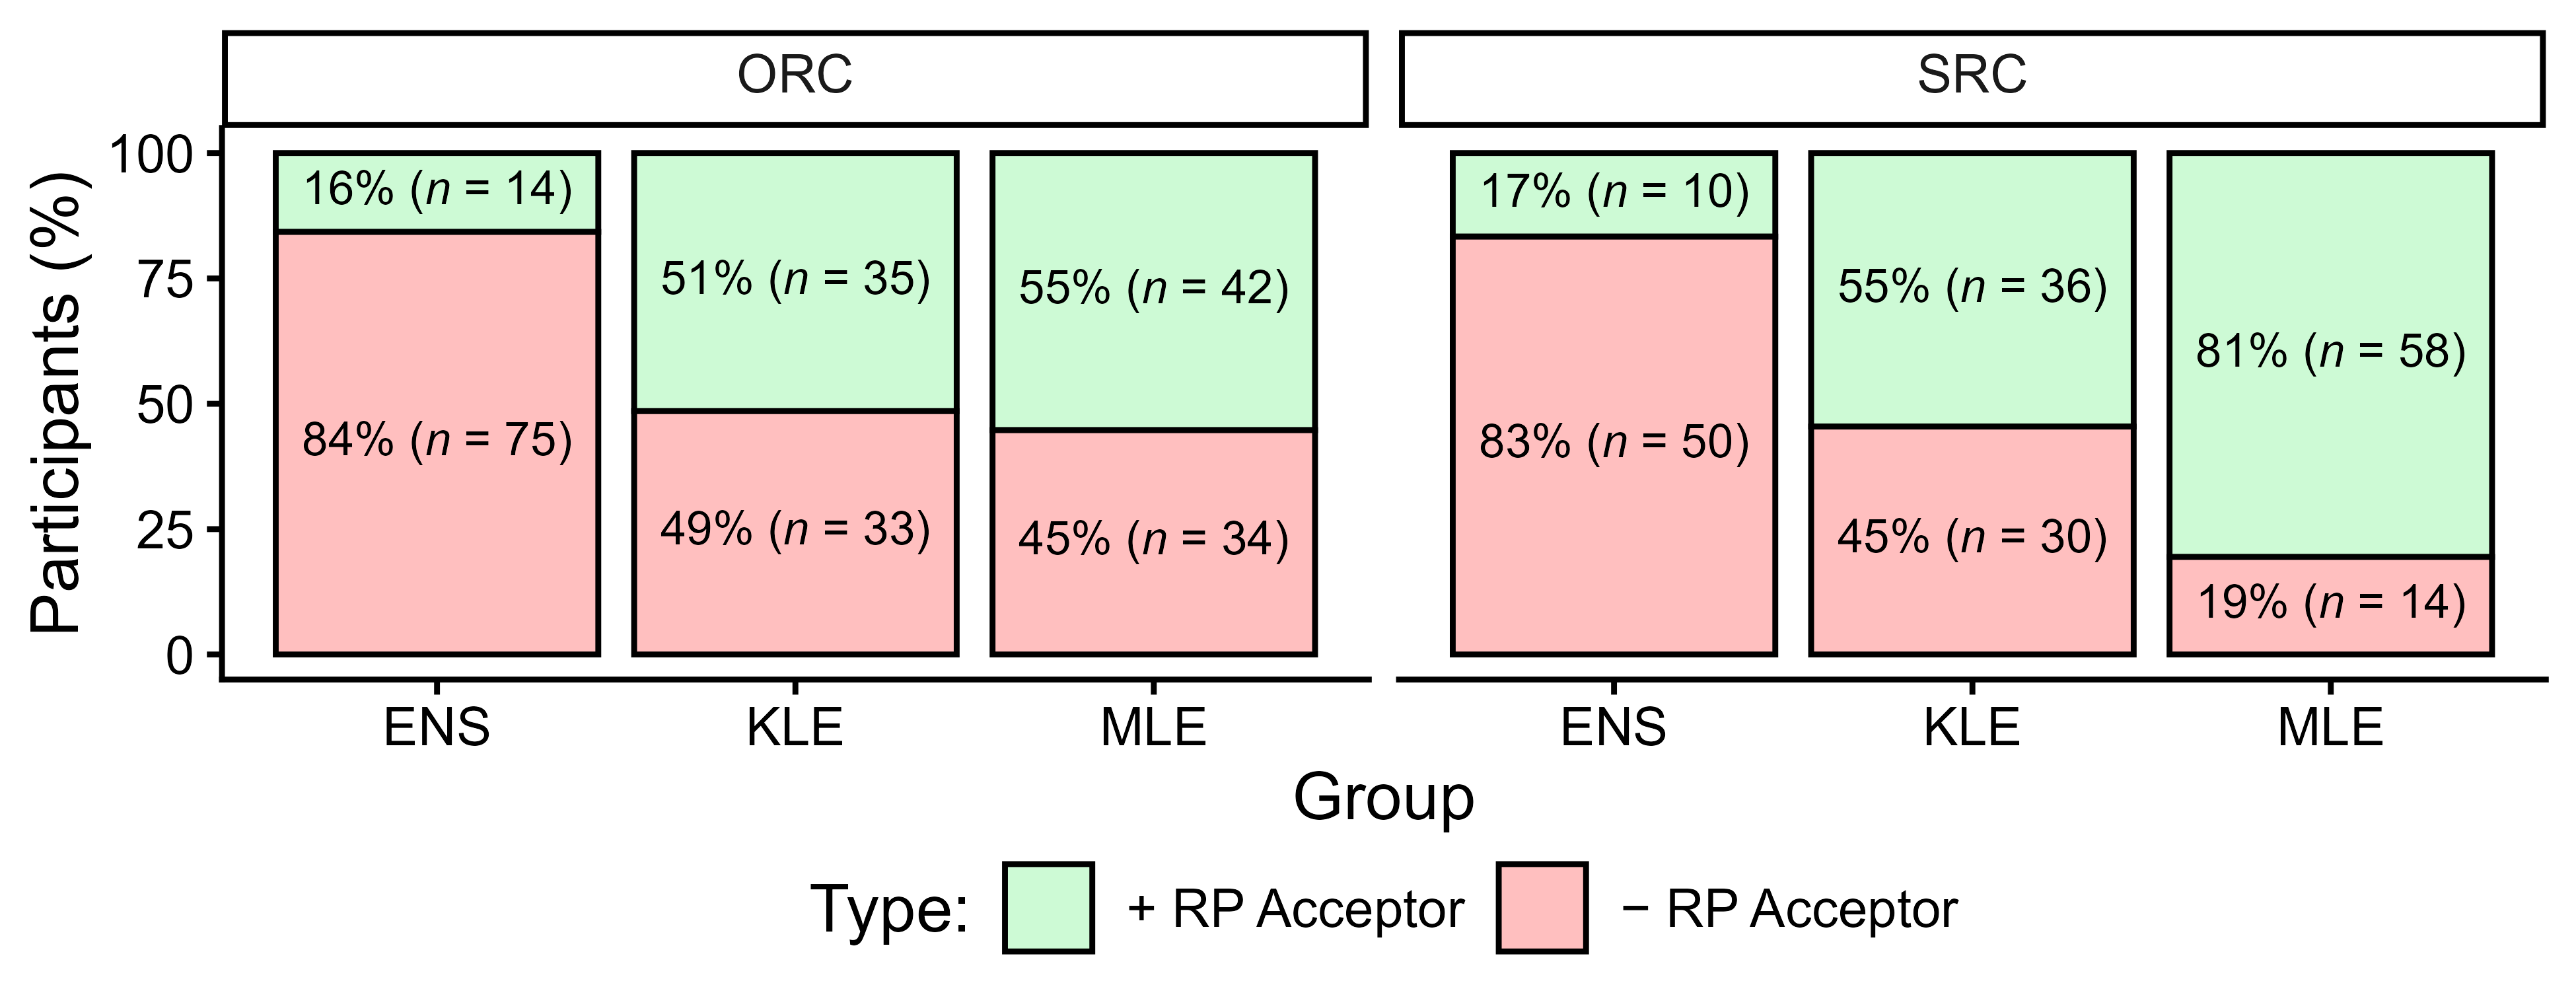
\includegraphics[width=\textwidth]{../analysis/plots/ajt_subgroup_acceptor.png}
\vspace{-34pt}
\end{figure}

\noindent RP acceptors were rare among the native speaker controls, amounting to 16\% of ENSs in the ORC dataset and 17\% of ENSs in the SRC dataset. In almost all cases, these ENSs accepted RPs only in the Island condition. RP acceptance was much more common among L2ers, with over 50\% of KLEs and MLEs in each study qualifying as RP acceptors. MLEs in the SRC dataset had the highest rates of RP acceptance, with 81\% qualifying as RP acceptors. Removing RP acceptors left 142 participants in the ORC dataset (ENS: 75; KLE: 33; MLE: 34) and 94 participants in the SRC dataset (ENS: 50; KLE: 30; MLE: 14).

%========================================================%
\section{Reanalysis of the EPT response data}\label{rnl-ept-token}
%========================================================%

Let us first consider RQ1, which asks how, with RP acceptors removed, processing strain affects rates of resumptive RCs in the EPT. Five participants from the English AJT dataset could not be included in this analysis because their EPT responses were either missing or had been excluded, as shown in Table~\ref{tab:rnl-spr-rt}.

\begin{table}
\caption{RP non-acceptors missing/excluded or retained in the elicited production tasks}\label{tab:rnl-ept-token}
\raggedright\setstretch{1}
\begin{tblr}{colspec = {lX[c]X[c]X[c]X[c]X[c]X[c]}, cell{1}{2,5} = {c=3}{}} 
\toprule 
& Missing/Excluded & & & Retained & & & \\
\cmidrule[lr]{2-4} \cmidrule[lr]{5-7}
Study & ENS & KLE & MLE & ENS & KLE & MLE \\ 
\midrule 
ORC & 1 & 2 & 1 & 74 & 31 & 33 \\
SRC & 1 & 0 & 0 & 49 & 30 & 14 \\
\bottomrule
\end{tblr}
\vspace{-12pt}
\end{table}

Figures~\ref{fig:ept-token-subgroup-orc} and \ref{fig:ept-token-subgroup-src} show the mean EPT responses for RP non-acceptors in, respectively, the ORC data and the SRC data. The rate of resumption responses appeared to increase down the SLW hierarchy in each combination of \textsc{group} and \textsc{subgroup}, suggesting that the processing advantage conferred by resumption in difficult-to-process RCs was not reserved only for RP acceptors.

\begin{figure}
\caption{Mean responses for RP non-acceptors in the ORC elicited production task} \label{fig:ept-token-subgroup-orc}
\raggedright\setstretch{1}
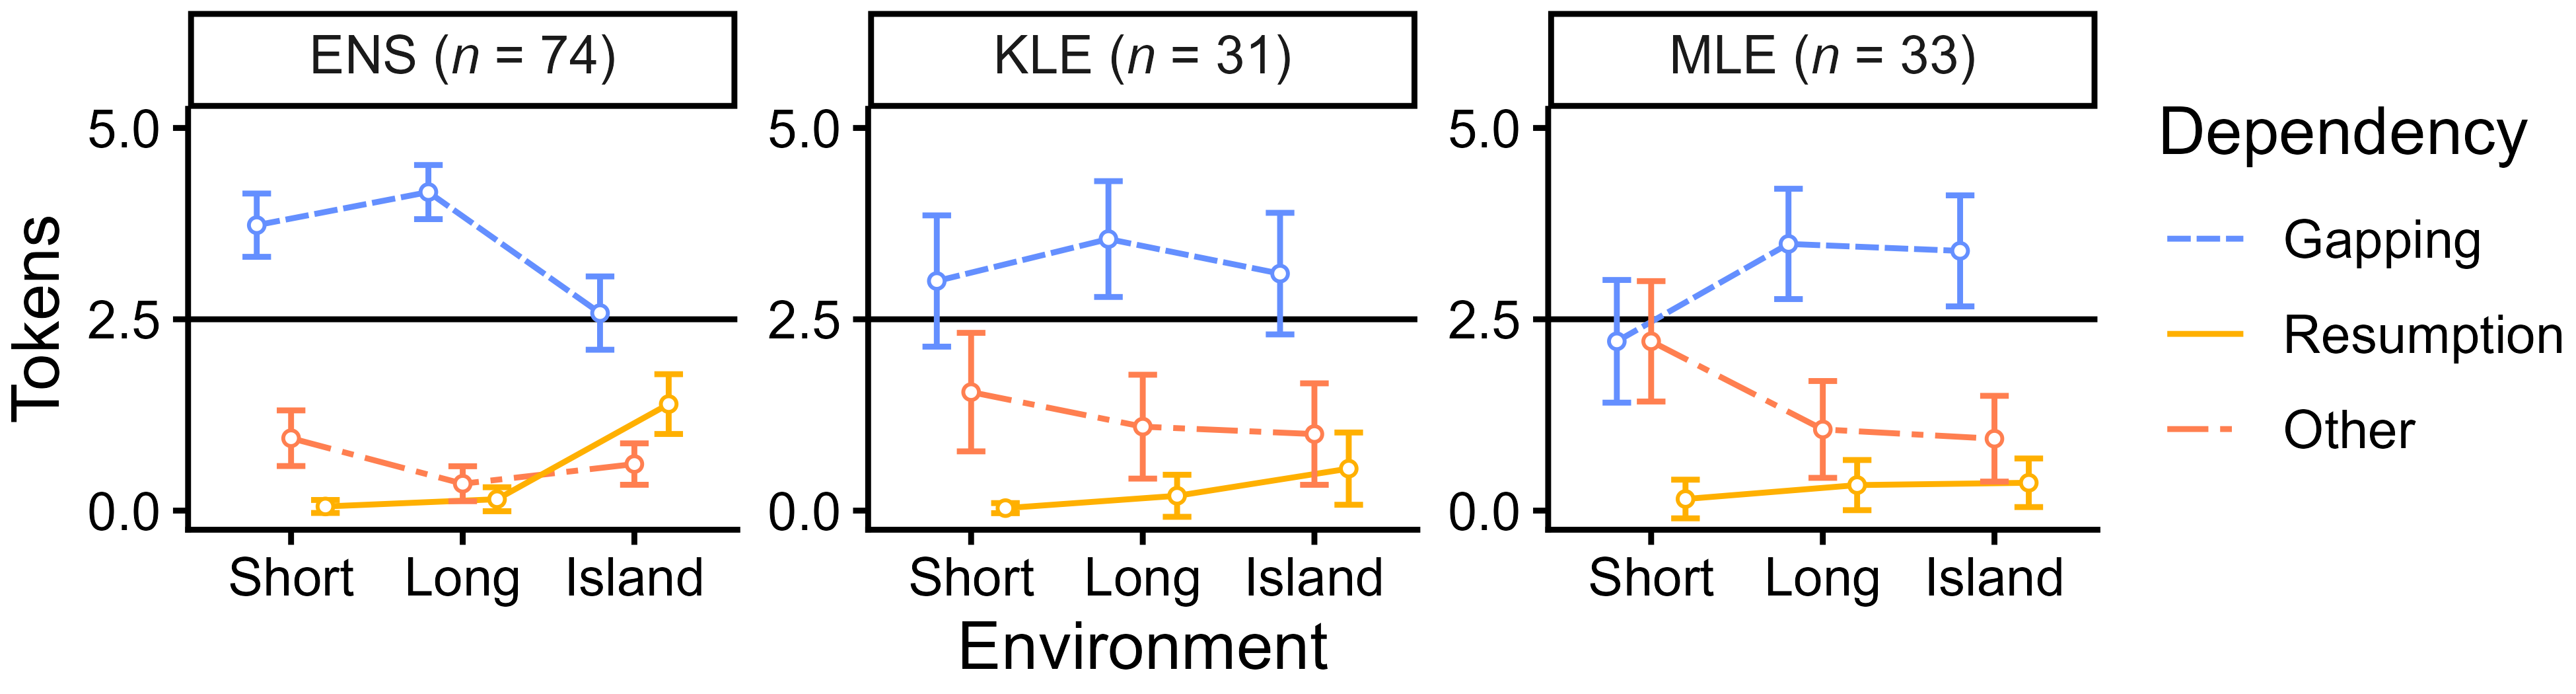
\includegraphics[width=\textwidth]{../analysis/plots/orc_ept_token_nonacceptor.png}
\textit{Note}. Max = 5 tokens per condition; error bars are 95\% \textit{CI}s; center line represents 50\% of responses; nontarget responses\footnotemark{} are omitted.
\vspace{-12pt}
\end{figure}

\footnotetext{As a reminder, nontarget responses were those for which the participant failed to produce an RC or to reference information from the sentences in the trial.}

\begin{figure}
\caption{Mean responses for RP non-acceptors in the SRC elicited production task} \label{fig:ept-token-subgroup-src}
\raggedright\setstretch{1}
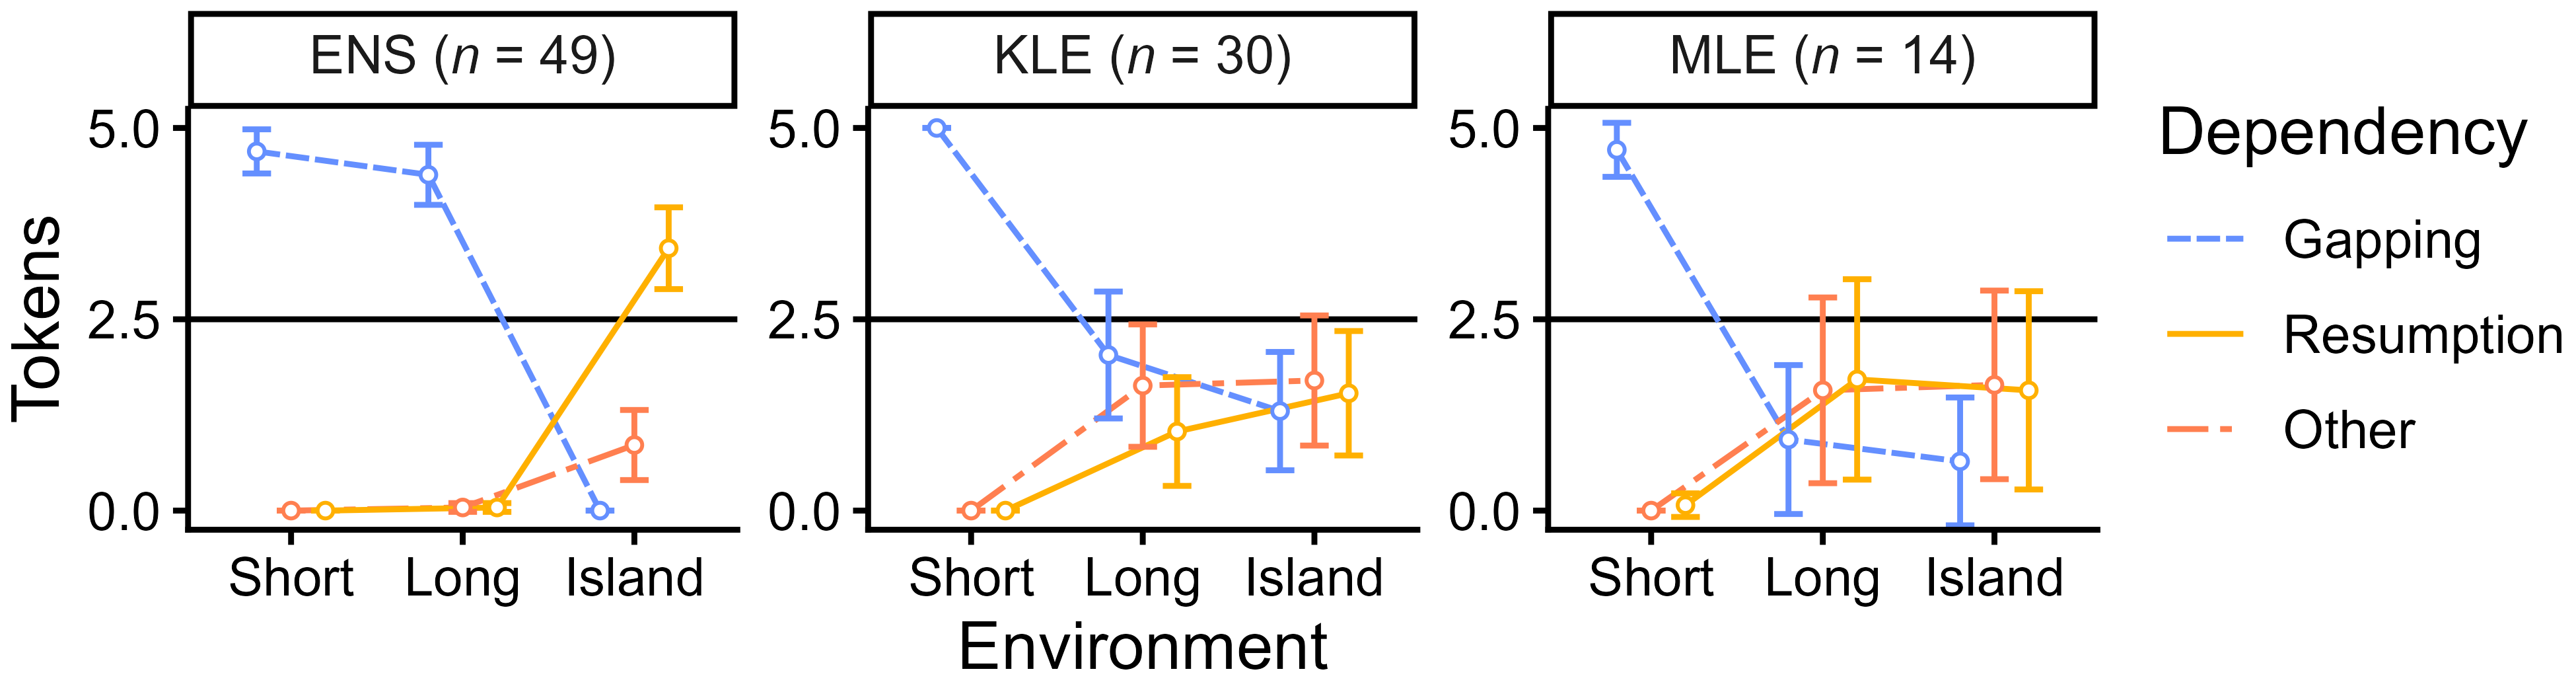
\includegraphics[width=\textwidth]{../analysis/plots/src_ept_token_nonacceptor.png}
\textit{Note}. Max = 5 tokens per condition; error bars are 95\% \textit{CI}s; center line represents 50\% of responses; nontarget responses are omitted.
\vspace{-12pt}
\end{figure}

To further examine the resumption rates among RP non-acceptors, I~fit their binary [\textsc{±resumption}] responses (Resumption = [\textsc{+resumption}]; Gapping = [\textsc{−resumption}]; Other = [\textsc{−resumption}]; Nontarget = [\textsc{−resumption}]) to separate mixed-effects logistic regression models for the ORC and SRC datasets. 

The ORC model (model formula: \textsc{resumption \~{} environment * group + (1 | participant) + (1 + group | item)}---see Appendix~\ref{app-results-reanalysis}, Table~\ref{tab:app-orc-ept-token-subgroup-model} for details) yielded a significant effect for \textsc{environment}, with the Long and Island conditions having more resumption responses than the Short condition (Long~−~Short: $\hat{\beta}$~=~1.86, \textit{SE}~=~0.58 $p$~=~.001; Island~−~Short: $\hat{\beta}$~=~3.91, \textit{SE}~=~0.59, $p$~<~.001). The two-way \textsc{environment}[Island~−~Short] × \textsc{group}[MLE~−~ENS] interaction also came out as significant ($\hat{\beta}$~=~−3.94, \textit{SE}~=~1.06, $p$~<~.001), indicating that the [Island~−~Short] contrast in the rate of resumption responses was larger for ENSs than for MLEs. In the pairwise comparisons, the [Island~−~Short] and [Island~−~Long] contrasts came out as significant for both ENSs (Island~−~Short: $\hat{\beta}$~=~5.45, \textit{SE}~=~0.74, $p$~<~.001; Island~−~Long: $\hat{\beta}$~=~3.94, \textit{SE}~=~0.47, $p$~<~.001) and KLEs (Island~−~Short: $\hat{\beta}$~=~4.76, \textit{SE}~=~1.38, $p$~=~.005; Island~−~Long: $\hat{\beta}$~=~2.08, \textit{SE}~=~0.75, $p$~=~.042). None of the contrasts was found to be significant for the MLE group.

For the SRC dataset, there were no Short-condition resumption responses among ENSs and KLEs; I~dealt with this absence of observations by adding two dummy participants, one ENS and one KLE, who gave only resumption responses across all conditions. The model fit to this modified dataset (model formula: \textsc{resumption \~{} environment * group + (1 | participant) + (1 | item)}---see Appendix~\ref{app-results-reanalysis}, Table~\ref{tab:app-src-ept-token-subgroup-model} for details) found (a)~a significant effect for \textsc{environment}, with the Long and Island conditions having more resumption responses than the Short condition (Long~−~Short: $\hat{\beta}$~=~6.16, \textit{SE}~=~1.30, $p$~<~.001; Island~−~Short: $\hat{\beta}$~=~11.37, \textit{SE}~=~1.95, $p$~<~.001), and (b)~a marginally significant effect for \textsc{group}, with KLEs having lower rates of resumption than ENSs ($\hat{\beta}$~=~−4.82, \textit{SE}~=~2.91, $p$~=~.098). Several of the two-way interactions involving \textsc{environment} and \textsc{group} were also in the marginal-to-significant range. Pairwise comparisons did not find significant either the [Long~−~Short] contrast for ENSs ($p$~=~.846) or the [Island~−~Long] contrast for MLEs ($p$~=~.965); however, all the other contrasts came out as significant ($p$~<~.05), with resumption rates increasing down the SLW hierarchy.

To review, rates of resumption responses increased numerically down the SLW hierarchy for all groups, (even) after RP acceptors had been removed. These increases were found to be statistically meaningful for each group in at least the SRC study (ENSs, KLEs, and MLEs) if not also the ORC study (ENSs and KLEs). This pattern of English results indicates that for native speaker and L2er alike, one need not consider resumption acceptable to derive a processing benefit from it during RC production.

%========================================================%
\section{Reanalysis of the SPRT region-of-interest RT data}\label{rnl-spr-rt}
%========================================================%

Next, let us consider RQ2, which asks how, with RP acceptors removed, resumption in RCs affects RTs at the regions of interest in the SPRT. Again, five participants from the English AJT dataset could not be included in this analysis because their SPRT data were either missing or had been excluded, as shown in Table~\ref{tab:rnl-spr-rt}.

\begin{table}
\caption{RP non-acceptors missing/excluded or retained in the self-paced reading tasks}\label{tab:rnl-spr-rt}
\raggedright\setstretch{1}
\begin{tblr}{colspec = {lX[c]X[c]X[c]X[c]X[c]X[c]}, cell{1}{2,5} = {c=3}{}} 
\toprule 
& Missing/Excluded & & & Retained & & \\
\cmidrule[lr]{2-4} \cmidrule[lr]{5-7}
Study & ENS & KLE & MLE & ENS & KLE & MLE \\ 
\midrule 
ORC & 0 & 1 & 4 & 75 & 32 & 30 \\
SRC & 0 & 0 & 0 & 50 & 30 & 14 \\
\bottomrule
\end{tblr}
\vspace{-12pt}
\end{table}

For this analysis, I~focused on the regions where the processing effect for resumption was strongest: Region~1 in the ORC dataset and Region~2 in the SRC dataset (see~Section~\ref{spr-rt-proficiency}). Figures~\ref{fig:spr-rt-subgroup-orc} and \ref{fig:spr-rt-subgroup-src} show the mean log-transformed RTs for RP non-acceptors in, respectively, the ORC data and the SRC data. In each group, there was a numerical advantage for RPs relative to gaps in the Long and/or Island conditions, suggesting that processing facilitation for RPs was not restricted to RP acceptors.

\begin{figure}
\caption{Mean log RTs at Region 1 for RP non-acceptors in the ORC self-paced reading task} \label{fig:spr-rt-subgroup-orc}
\raggedright\setstretch{1}
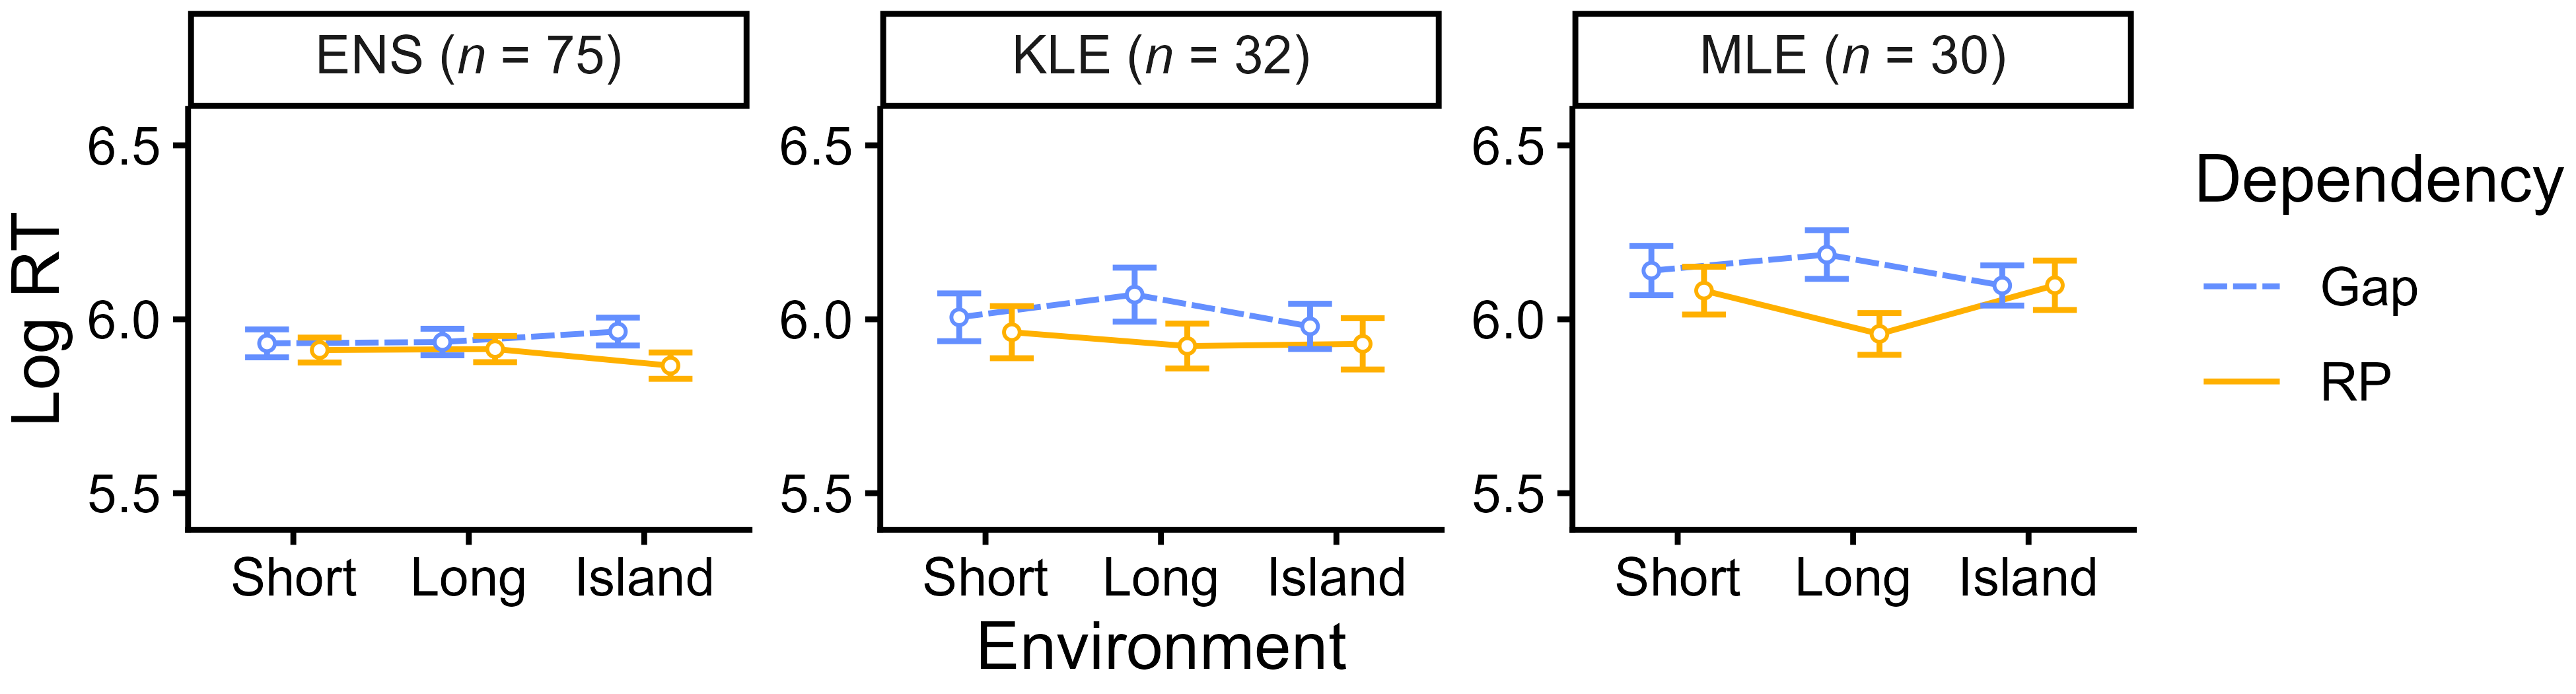
\includegraphics[width=\textwidth]{../analysis/plots/orc_spr_rt_nonacceptor.png}
\textit{Note}. Error bars are 95\% \textit{CI}s.
\vspace{-12pt}
\end{figure}

\begin{figure}
\caption{Mean log RTs at Region 2 for RP non-acceptors in the SRC self-paced reading task} \label{fig:spr-rt-subgroup-src}
\raggedright\setstretch{1}
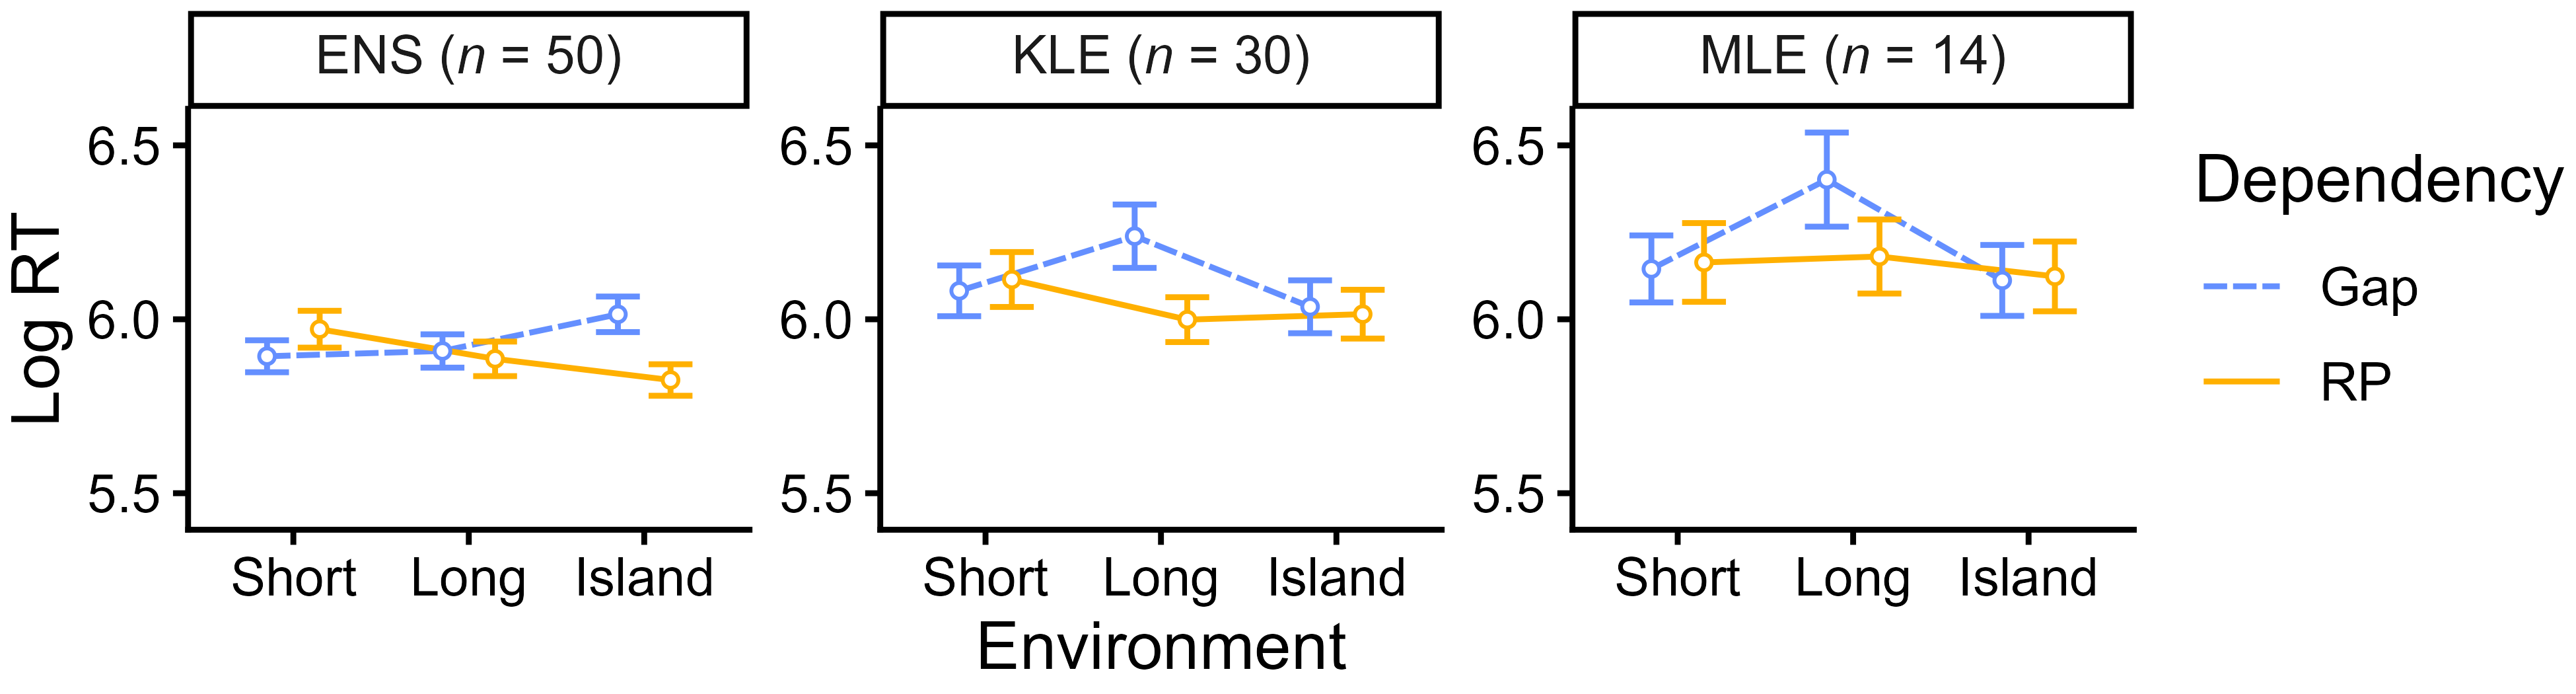
\includegraphics[width=\textwidth]{../analysis/plots/src_spr_rt_nonacceptor.png}
\textit{Note}. Error bars are 95\% \textit{CI}s.
\vspace{-12pt}
\end{figure}

I~examined the log RTs for RP non-acceptors in more detail by fitting them to separate linear mixed-effects models for the ORC and SRC datasets. 

The ORC model (model formula: \textsc{log rt \~{} dependency * environment * group + (1 + dependency + environment | participant) + (1 + dependency + environment + group | item)}---see Appendix~\ref{app-results-reanalysis}, Table~\ref{tab:app-orc-spr-logrt-subgroup-model} for details) found significant effects for (a)~\textsc{dependency}, with RP trials having faster RTs than gap trials (RP~−~Gap: $\hat{\beta}$~=~−0.05, \textit{SE}~=~0.01, $p$~<~.001), and (b)~\textsc{group}, with MLEs having slower RTs than ENSs (MLE~−~ENS: $\hat{\beta}$~=~0.14, \textit{SE}~=~0.04, $p$~=~.001). Several of the two-way and three-way interactions were also significant ($p$~>~.05). Pairwise comparisons revealed that the RP advantage in RTs was significant in the Long condition for KLEs and MLEs (KLE: $\hat{\beta}$~=~−0.15, \textit{SE}~=~0.03, $p$~<~.001; MLE: $\hat{\beta}$~=~−0.14, \textit{SE}~=~0.03, $p$~<~.001) and in the Island condition for ENSs ($\hat{\beta}$~=~−0.09, \textit{SE}~=~0.02, $p$~<~.001).

The SRC model (model formula: \textsc{log rt \~{} dependency * environment * group + (1 + dependency * environment | participant) + (1 + dependency + environment | item)}---see Appendix~\ref{app-results-reanalysis}, Table~\ref{tab:app-src-spr-logrt-subgroup-model} for details) found (a)~a significant effect for \textsc{dependency}, with RP trials having faster RTs than gap trials ($\hat{\beta}$~=~−0.06, \textit{SE}~=~0.02, $p$~<~.001), (b)~a marginal-to-significant effect for \textsc{environment}, both with the Long condition having slower RTs than the Short condition ($\hat{\beta}$~=~0.04, \textit{SE}~=~0.02, $p$~<~.030) and with the Island condition having faster RTs than the Short condition ($\hat{\beta}$~=~−0.04, \textit{SE}~=~0.02, $p$~=~.063), and (c) a significant effect for \textsc{group}, with KLEs and MLEs both having slower RTs than ENSs (KLE~−~ENS: $\hat{\beta}$~=~0.16, \textit{SE}~=~0.06, $p$~=~.011; MLE~−~ENS: $\hat{\beta}$~=~0.26, \textit{SE}~=~0.08, $p$~=~.002). Several of the two-way and three-way interactions were also significant ($p$~<~.05). As with the ORC model, pairwise comparisons revealed that RP trials were significantly faster than gap trials in the Long condition for KLEs and MLEs (KLE: $\hat{\beta}$~=~−0.23, \textit{SE}~=~0.05, $p$~<~.001; MLE: $\hat{\beta}$~=~−0.21, \textit{SE}~=~0.06, $p$~=~.014) and in the Island condition for ENSs ($\hat{\beta}$~=~−0.19, \textit{SE}~=~0.03, $p$~<~.001).

Overall, these results show that the RP advantage in RTs observed in the SPRT data persists (even) with RP acceptors removed from the analysis. This in turn suggests that processing facilitation associated with resumption during RC comprehension is not limited to RP acceptors, again for both native speakers and L2ers. 

%========================================================%
\section{Reanalysis of the SPRT comprehension-question accuracy data}\label{rnl-spr-accuracy}
%========================================================%

Finally, we come to RQ3, which asks how, with RP acceptors removed, resumption affects comprehension-question accuracy in the SPRT. The participant counts for this analysis were the same as for the RT analysis in the previous section. Figures~\ref{fig:spr-accuracy-subgroup-orc} and \ref{fig:spr-accuracy-subgroup-src} show the mean accuracy scores on comprehension questions for RP non-acceptors in, respectively, the ORC data and the SRC data. There was an uninterrupted numerical advantage for RPs in all groups, indicating that resumption assists with accurate RC interpretation even for RP non-acceptors. The RP-over-gap advantage tended to be larger in the Long and/or Island conditions than in the Short condition, suggesting that the helpfulness of resumption increases down the SLW hierarchy.

\begin{figure}
\caption{Mean comprehension-question accuracy for RP non-acceptors in the ORC self-paced reading task} \label{fig:spr-accuracy-subgroup-orc}
\raggedright\setstretch{1}
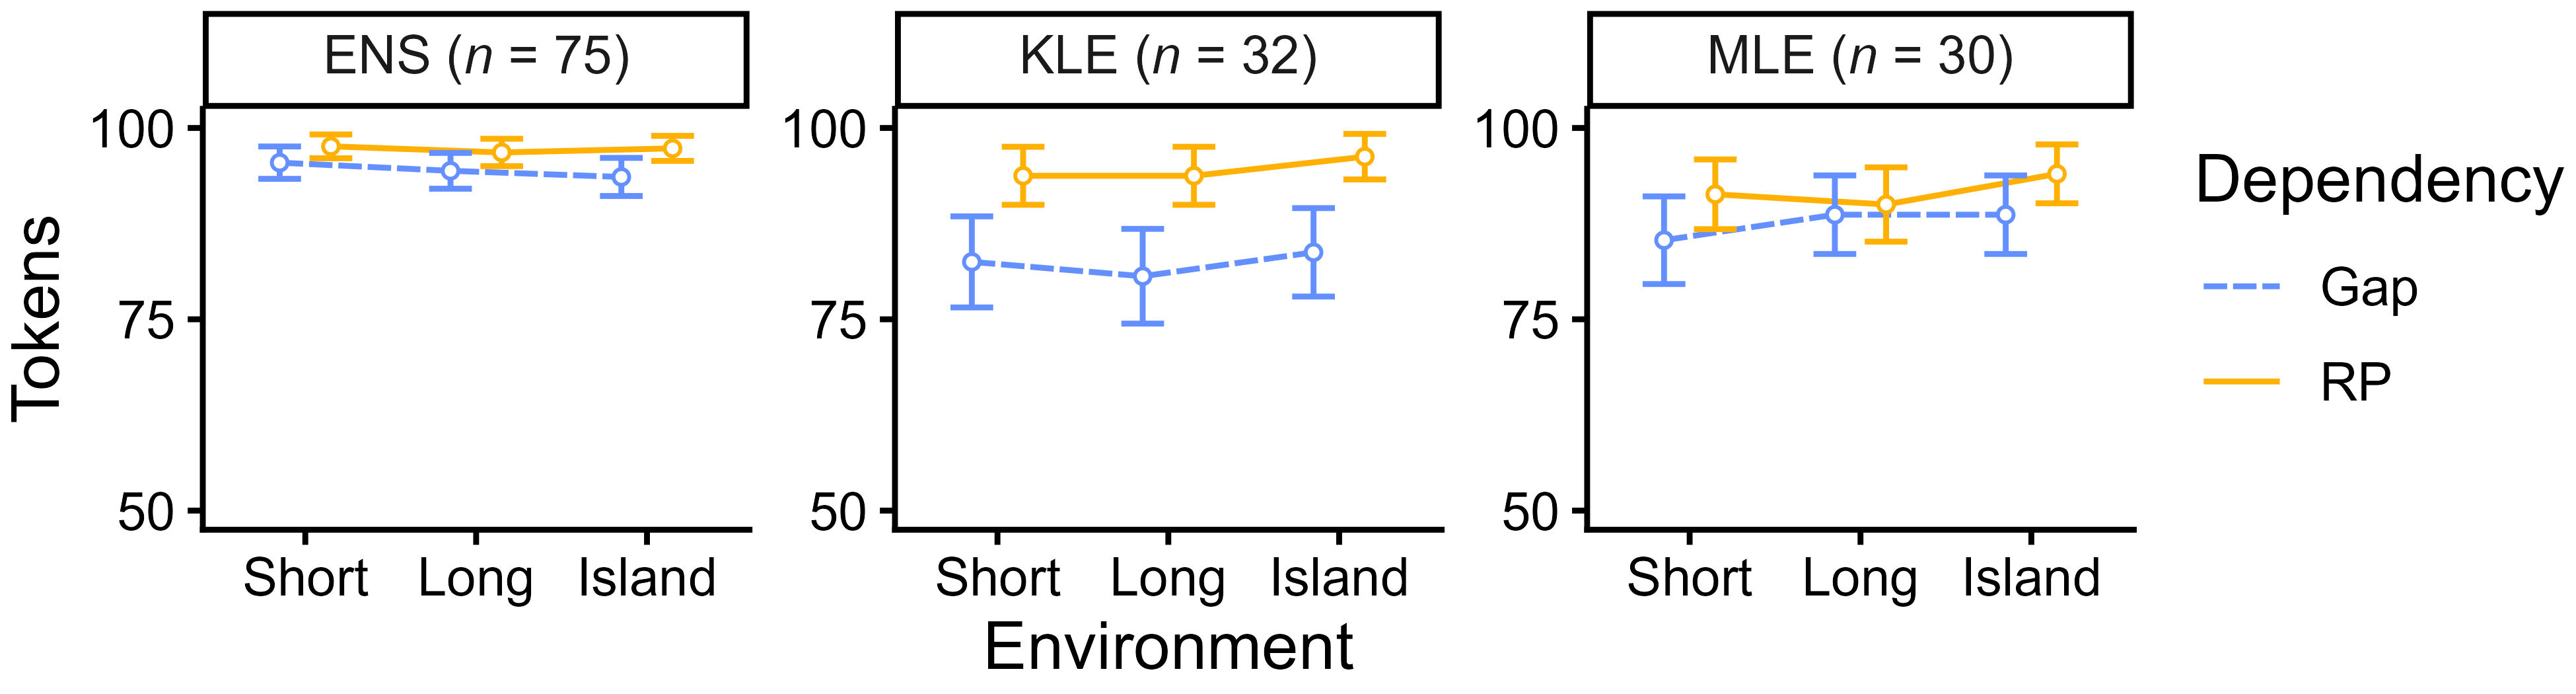
\includegraphics[width=\textwidth]{../analysis/plots/orc_spr_accuracy_nonacceptor.png}
\textit{Note}. Error bars are 95\% \textit{CI}s.
\vspace{-12pt}
\end{figure}

\begin{figure}
\caption{Mean comprehension-question accuracy for RP non-acceptors in the SRC self-paced reading task} \label{fig:spr-accuracy-subgroup-src}
\raggedright\setstretch{1}
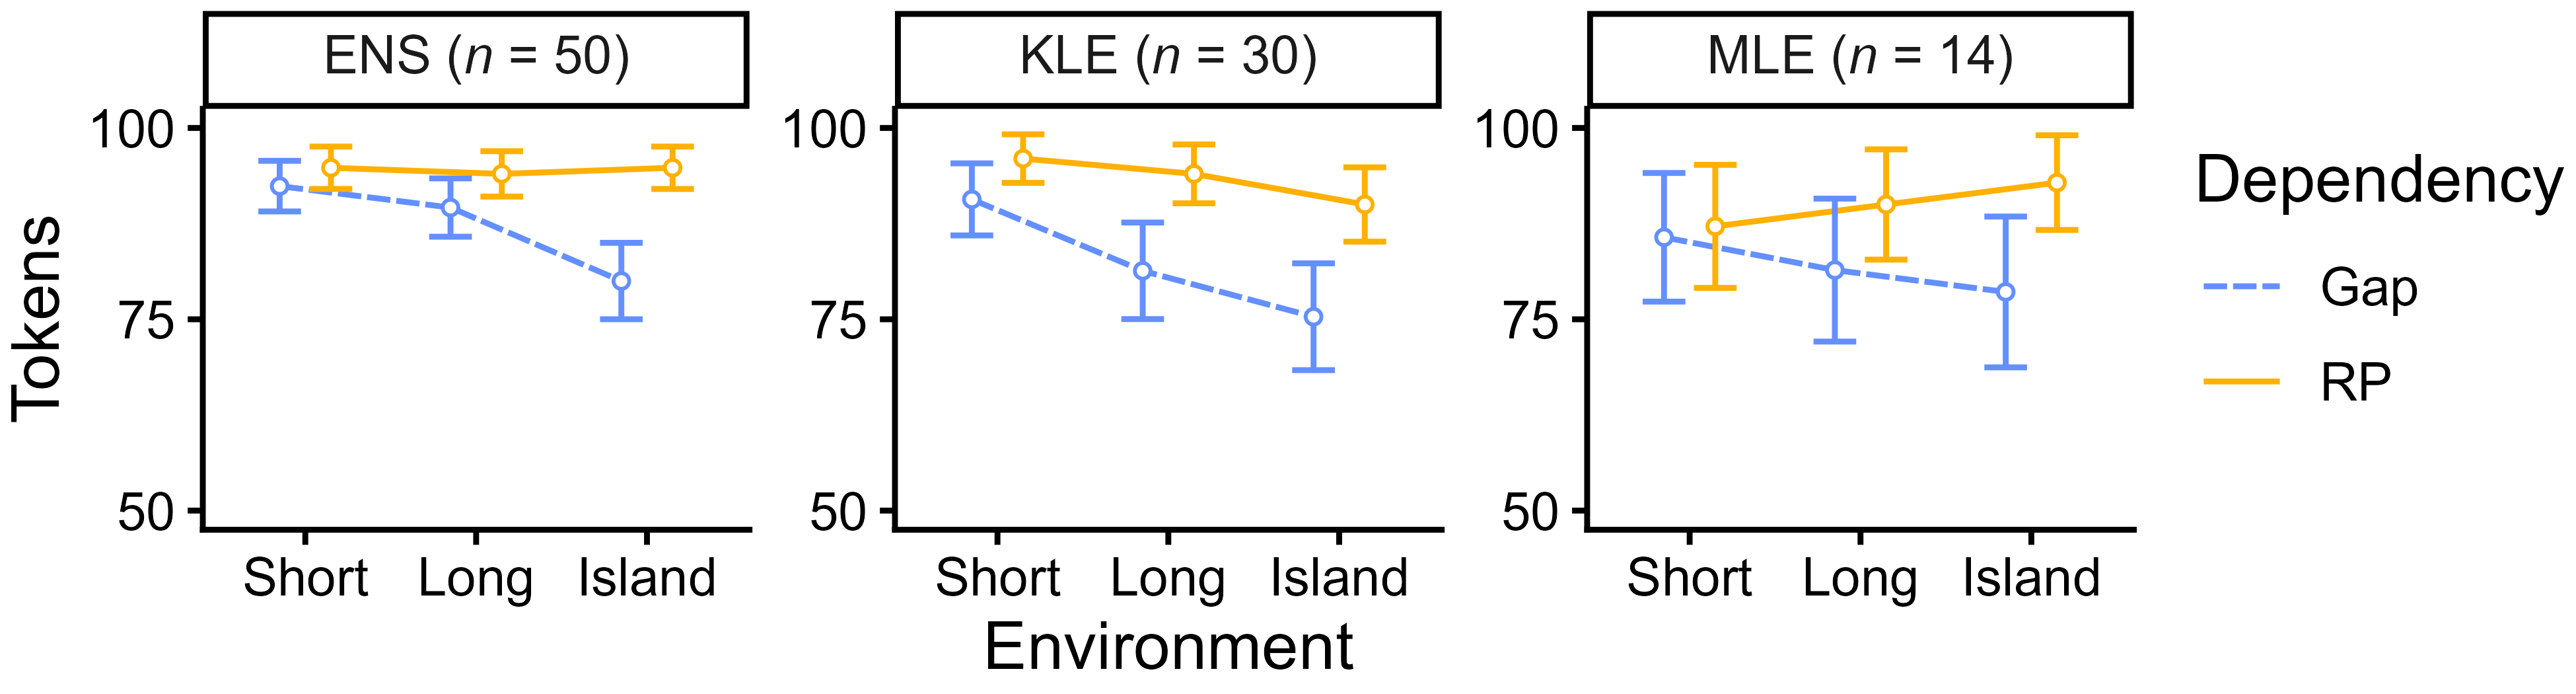
\includegraphics[width=\textwidth]{../analysis/plots/src_spr_accuracy_nonacceptor.png}
\textit{Note}. Error bars are 95\% \textit{CI}s.
\vspace{-12pt}
\end{figure}

I~further analyzed the binary comprehension-question accuracy scores for RP non-acceptors via separate mixed-effects logistic regression models for the ORC and SRC datasets. 

The ORC model (model formula: \textsc{accuracy \~{} dependency * environment * group + (1 + dependency * environment | participant) + (1 + dependency + environment + group | item)}---see Appendix~\ref{app-results-reanalysis}, Table~\ref{tab:app-orc-spr-accuracy-subgroup-model} for details) turned up significant effects for (a)~\textsc{dependency}, with RPs having higher accuracy than gaps (RP~−~Gap: $\hat{\beta}$~=~1.01, \textit{SE}~=~0.32, $p$~<~.001), and (b)~\textsc{group}, with KLEs and MLEs both having lower accuracy than ENSs (KLE~−~ENS: $\hat{\beta}$~=~−1.27, \textit{SE}~=~0.34, $p$~<~.001; MLE~−~ENS: $\hat{\beta}$~=~−0.97, \textit{SE}~=~0.37, $p$~=~.008). The \textsc{dependency}[RP~−~Gap] × \textsc{group}[KLE~−~ENS] interaction also came out as significant ($\hat{\beta}$~=~0.98, \textit{SE}~=~0.40, $p$~=~.014), indicating that the [RP~−~Gap] contrast was larger for KLEs than for ENSs. Pairwise comparisons showed that the RP-over-gap advantage in accuracy scores was in the marginal-to-significant range only for KLEs, and only in the Long and Island conditions (Long: $\hat{\beta}$~=~1.90, \textit{SE}~=~0.65, $p$~=~.028; Island: $\hat{\beta}$~=~2.02, \textit{SE}~=~0.75, $p$~=~.059). The [RP~−~Gap] contrast was not found to be significant for ENSs or MLEs in any environments in this analysis, perhaps due to (a)~ceiling effects in the ENS group and (b)~reduced sample size in the MLE group.

The SRC model (model formula: \textsc{accuracy \~{} dependency * environment * group + (1 + dependency * environment | participant) + (1 + dependency * environment + group | item)}---see Appendix~\ref{app-results-reanalysis}, Table~\ref{tab:app-src-spr-accuracy-subgroup-model} for details) found significant effects for (a)~\textsc{dependency}, with RPs having higher accuracy than gaps ($\hat{\beta}$~=~1.66, \textit{SE}~=~0.34, $p$~<~.001), and (b)~\textsc{environment}, with the Island condition having lower accuracy than the Short condition ($\hat{\beta}$~=~−0.99, \textit{SE}~=~0.44, $p$~=~.025). None of the interaction terms came out as significant, indicating that the size of each of these effects did not vary in a statistically meaningful way across levels of the other variables.

In short, there was a strong tendency for accuracy to be higher for RPs than for gaps, especially at lower levels on the SLW hierarchy, where processing should be more challenging. That this pattern of results held even when RP acceptors were removed from the dataset indicates, once again, that processing benefits associated with resumption during English RC comprehension are not dependent upon RP acceptance, for either native speakers or L2ers.

%========================================================%
\section{Summing up}\label{rnl-conclusion}
%========================================================%

This chapter set out to test whether the group processing effects for resumption observed in the EPT and SPRT data (see~Chapters~\ref{ch-ept} and \ref{ch-spr}) were due to an oversized effect from the RP acceptors. After removal of those RP acceptors, reanalysis of the EPT response data, the SPRT region-of-interest RT data, and the SPRT comprehension-question accuracy data all pointed to RPs easing processing of RCs under processing strain. These English results indicate that L1 and L2 participants were able to benefit from the processing facilitation conferred by resumption even if they did not consider RPs to be acceptable in English RCs. Furthermore, the fact that many participants produced resumptive RCs in the EPT while not accepting them in the English AJT indicates that production patterns do not necessarily reflect representations licensed by the grammar, in contradiction of assumptions made by \textcite{hyltenstam1984,hyltenstam1990}, \textcite{eckman2004}, and many others in the traditional L2 literature.